\documentclass[twocolumn]{article}
\usepackage[utf8]{inputenc}
\usepackage{biblatex}
\usepackage{listings}
\usepackage{graphicx}
\usepackage{tabularx}
\usepackage{xcolor}
\usepackage[toc,page]{appendix}
\usepackage{setspace}

% \setstretch{1.5}

\definecolor{codegreen}{rgb}{0,0.6,0}
\definecolor{codegray}{rgb}{0.5,0.5,0.5}
\definecolor{codepurple}{rgb}{0.58,0,0.82}
\definecolor{backcolour}{rgb}{0.95,0.95,0.92}

\lstdefinestyle{mystyle}{
    backgroundcolor=\color{backcolour},
    commentstyle=\color{codegreen},
    keywordstyle=\color{magenta},
    numberstyle=\tiny\color{codegray},
    stringstyle=\color{codepurple},
    basicstyle=\ttfamily\footnotesize,
    breakatwhitespace=true,
    breaklines=true, 
    captionpos=b,
    keepspaces=true, 
    numbers=left,
    numbersep=3pt,
    showspaces=false,
    showstringspaces=false,
    showtabs=false,
    tabsize=2
}
\lstset{style=mystyle}

\lstdefinelanguage
   [x64]{Assembler}     % add a "x64" dialect of Assembler
   [x86masm]{Assembler} % based on the "x86masm" dialect
   % with these extra keywords:
   {morekeywords={CDQE,CQO,CMPSQ,CMPXCHG16B,JRCXZ,LODSQ,MOVSXD, %
                  POPFQ,PUSHFQ,SCASQ,STOSQ,IRETQ,RDTSCP,SWAPGS, %
                  rax,rdx,rcx,rbx,rsi,rdi,rsp,rbp, %
                  r8,r8d,r8w,r8b,r9,r9d,r9w,r9b, %
                  r10,r10d,r10w,r10b,r11,r11d,r11w,r11b, %
                  r12,r12d,r12w,r12b,r13,r13d,r13w,r13b, %
                  r14,r14d,r14w,r14b,r15,r15d,r15w,r15b}} % etc.

\newcommand{\code}[1]{\texttt{#1}}
\newcommand{\miniheading}[1]{\noindent\makebox[\columnwidth][l]{\textbf{#1}}}

\setlength{\columnsep}{15pt}

\graphicspath{ {./images/} }
\addbibresource{bibliography.bib}

\title{C Annotations for Concurrent Information Flow Security}
\author{Alexander Blyth}
\date{June 2021}

\begin{document}
\maketitle

\textbf{\textit{Abstract} - Information flow security in concurrency is difficult due to the increasing complexity introduced with multiple threads. Additionally, compiler optimisations can break security guarantees that have been verified in source code. In this paper, we propose a thesis to explore these issues through providing annotations in C source code that propagate through to the binary or assembly. These annotations could then be used to guide a static analysis of information flow security in concurrency. This approach involves (1) capturing C source code annotations provided by the user about the security policy of data and variables and (2) passing these annotations down to lower representations where static analysis tools can be utilised to identify security vulnerabilities in the produced binary. }

\section{Topic Definition}
This paper describes the motivation, background knowledge and plan for the proposed thesis \textit{Compiler Annotation Solutions for Concurrent Information Flow Security}.

There is a high degree of complexity in verifying security guarantees in concurrent programs \cite{mantel2014noninterference}\cite{smith2019value}\cite{vaughan2012secure}. Additionally, aggressive compiler optimisations can modify the binary output in unexpected ways \cite{d2015correctness}. To preserve the security of a program, the flow of sensitive information must be protected to avoid flowing in to untrusted sources \cite{balliu2014logics}. This is where static analysis tools can be used to verify the integrity of security guarantees and the flow of sensitive information. In this thesis, we look to explore a solution to information flow security in concurrent programs through analysing the output after aggressive compiler optimisations.

We propose a tool to analyse C programs to detect security violations in information flow control. This tool will preserve annotations provided by the programmer in source code through lowering passes and aggressive compiler optimisations. The tool will work alongside the \textit{Weakest Precondition for Information Flow} (wpif) transformer described by Winter et al. \cite{winter2020information} to allow the programmer to assess the security of information flow in their concurrent programs.

Similar tools for propagating annotations and properties through compiler optimisations have been explored \cite{vu2020secure} \cite{schommer2018embedded} \cite{leroy2016compcert}, however, these tools focus on either generic solutions for propagating properties or to assist the static analysis of the \textit{Worst Case Execution Time}.


% !TeX root = ./report.tex
\section{Background}
Vulnerabilities in software can lead to catastrophic consequences when manipulated by attackers. In an open-source cryptographic software library (OpenSSL) used by an estimated two-thirds of web servers \cite{heartbleed} a security flaw called Heartbleed was discovered. Secure secrets such as financial data, encryption keys, or anything else stored in the server's memory could be leaked. Normally, one would send a Heartbeat request with a text string payload and the length of the payload. For example, a message of ``hello'' could be sent with the length of the message, 5. However, due to a improper input validation (buffer over-read), one could send a length longer that the string they actually sent. This would cause the server to respond with the original message and anything that was in the allocated memory at the time, including any potentially sensitive information. An example of this is shown in figure \ref{fig:heartbleed} \cite{heartbleedimg}.

\begin{figure}
    \centering
    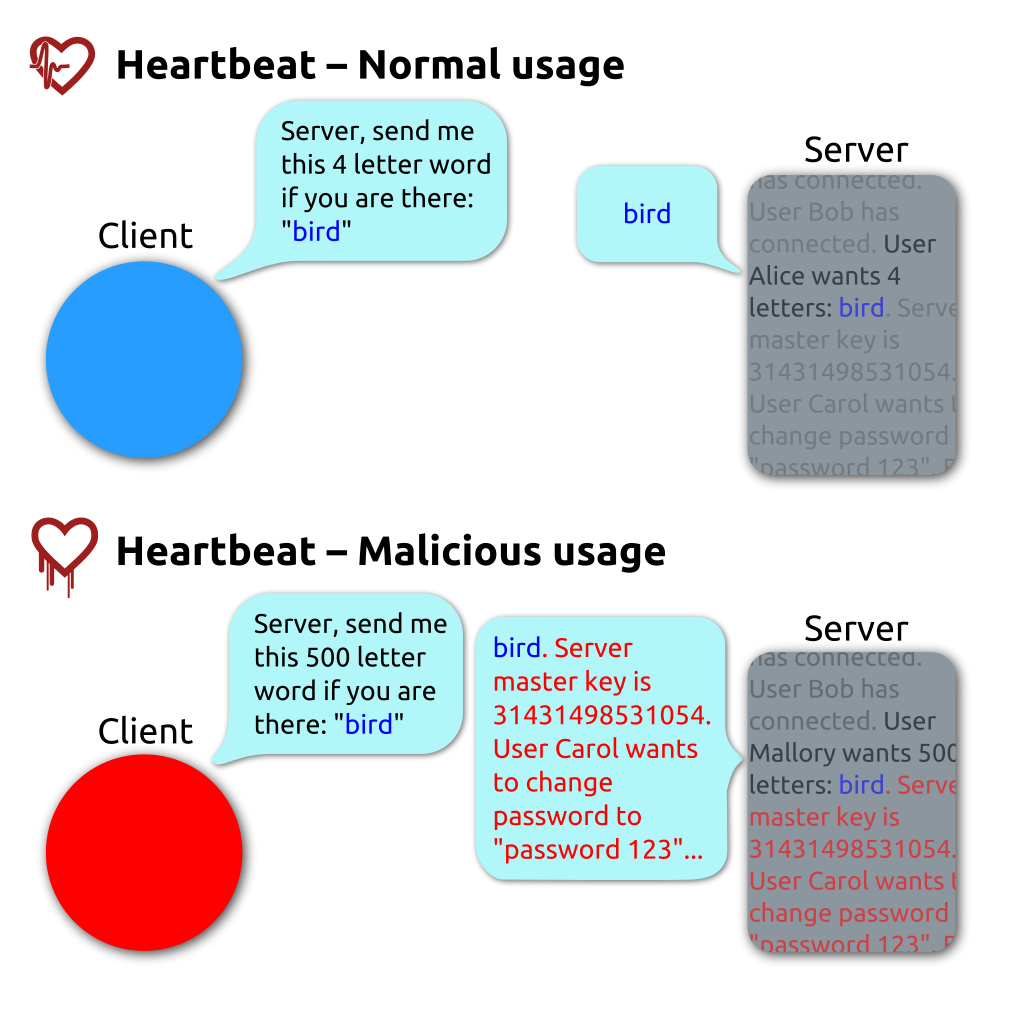
\includegraphics[width=\linewidth]{heartbleed.png}
    \caption{The Heartbleed bug. \cite{heartbleedimg}}
    \label{fig:heartbleed}
\end{figure}

Heartbleed was one of the most dangerous security bugs ever, and calls for major reflection by everyone in industry and research \cite{balliu2014logics}.

\subsection{Information Security}

Computer security is defined as a preservation of \textbf{integrity}, \textbf{availability} and \textbf{confidentiality} of information, and extends to include not only software but hardware, firmware, information, data and telecommunications \cite{guttman1995introduction}.
Confidentiality requires that data is not available to unauthorised users, and that individuals can control what information can be collected and disclosed to others. Data integrity requires that only authorised sources can modify data, and that the system can perform tasks without interference from outside sources. Finally, availability of a system requires that service is not denied to authorised users. Together, these principles create the CIA triad \cite{stallings2012computer}. To enforce a secure system, all three principles must be upheld.

Modern programs are becoming increasingly complex with potential for networking, multi-threading and storage permissions and more. As such, security mechanisms must be put in place to verify and enforce the information security requirements. The adequacy of a security mechanism depends on the adversary model. The adversary model is a formal definition of the attacker and their abilities in a system, and defines who we are protecting against \cite{do2019role}. Ideally we would like to design a system to protect against the strongest adversary or attacker, however, this is often not required or even possible. Instead, we must consider the security policy, security mechanism and strongest adversary model to make a system secure \cite{balliu2014logics}.

Standard security processes that handle access control such as a firewall or antivirus software can fail as they do not constrain where information is allowed to flow, meaning that once access is granted it can propagate to insecure processes where it can be accessed by attackers. Where a large system is being used, it is often the case that not all components of the codebase can be trusted, often containing potentially malicious code \cite{sabelfeld2003language}. Take for example your modern-day web project. Where a package manager such as Node Package Manager (npm) could be used to utilise open-source packages to speed up development progress, it could also inadvertently introduce security vulnerabilities. Rewriting all packages used to ensure security would be time-consuming and expensive and is not a viable option. Instead, controlling where information can flow and preventing secure data from flowing into untrusted sources or packages can maintain confidentiality of a system.

One may suggest runtime monitoring the flow of data to prevent leakage of secure data. Aside from the obvious computational and memory overhead, this method can have its own issues. Although it can detect an \textit{explicit} flow of data from a secure variable to a public variable, it is unable to detect \textit{implicit} data flow, where the state of secure data can be inferred from the state of public data or a public variable \cite{denning1977certification}. Take for example figure \ref{fig:implicit}. In this example, a public, readable variable is initially set to the value of 1. There is also a secret variable which may contain a key, password or some other secret that must be kept secure from any attackers. Depending on the value of the secret variable an attacker can infer information about this variable depending on whether the value of the public variable is updated to a value of 0. Assuming that the inner workings of the system is known by the attacker, information about the secret variable can be leaked \textit{implicitly} and inferred by the state of public variables.

\begin{figure}
    \begin{lstlisting}
secret := 0xC0DE mod 2
public := 1
if secret = 1
    public := 0
        \end{lstlisting}
    \caption{Implicit flow of data to a public variable}
    \label{fig:implicit}
\end{figure}

Security concerns do not only exist at the application level. In a huge codebase such as an OS, different low-level bugs can be exploited to gain access to data, such as by using buffer overflows to inject viruses or trojans \cite{agten2012recent}.

\subsection{Information Flow Control}
As seen by the issues that can be introduced via implicit and explicit flow of data, there is room to improve on the existing techniques imposed by current security measures. To protect confidentiality, secure or sensitive information must be prevented from flowing into public on insecure variables. Additionally, to protect integrity, untrusted data from public sources must be prevented from flowing into secure or trusted destinations \cite{balliu2014logics}. An information flow security policy can be introduced to classify or label data, or more formally, a set of \textit{security levels} to which each object is bound by across a multi-level security lattice \cite{denning1976lattice}. In this thesis, we will focus primarily on preserving confidentiality.

Many security levels can be identified to classify different classes of objects, however, for now we will consider two security levels: high and low. Data labelled as high signifies that the data is secret, and low data is classified as non-sensitive data, such that it does not need to be protected from an attacker or adversary. Variables that can hold data in a program can additionally be classified as high or low as a \textit{security classification}. A variable's security classification shows the highest classification of data it can safely contain \cite{winter2020information}. A high variable can hold both high and low data, whereas a low variable which is visible to an attacker can only safely hold low data. As mentioned previously, confidentiality must be upheld by preventing high or secret data from flowing to low or public variables where an attacker can observe it. The permitted flow of data can be observed in \ref{fig:flow}. Note that high data is not allowed to flow into low variables.

\begin{figure}
    
\includegraphics{flow.png}
    \caption{Permitted flow of data}
    \label{fig:flow}
\end{figure}

\subsection{Information Flow Security in Concurrency}
Controlling the flow of information is a difficult problem, however, this is only exacerbated in concurrent programs, which are a well known source of security issues \cite{mantel2014noninterference}\cite{smith2019value}\cite{vaughan2012secure}. Research has been conducted into concurrent programs to explore ways the security of concurrent programs can be verified. Mantel et al. \cite{mantel2011assumptions} introduced the concept of assumption and guarantee conditions, where assumptions are made about how concurrent threads access shared memory and guarantees are made about how an individual thread access shared memory that other threads may rely upon. Each thread can be observed individually using assumptions over the environment behaviour of other threads that can be then used to prove a guarantee about that individual thread. As two concurrent threads can interleave their steps and behaviour, there is a lot of complexity and possibilities for the overall behaviour. This concept of assumptions (or rely) and guarantee conditions can reduce the complexity of understanding interleaving behaviour in threads and assist in verifying the correctness of information flow security in concurrency. However, this approach is limited in the types of assumptions and guarantees it supports. Building on this, Murray et al. \cite{ernst2019seccsl} \cite{murray2018covern} provide information flow logic on how to handle dynamic, value-dependent security levels in concurrent programs. In this case, the security level of a particular variable may depend on one or more other variables in the program. As such, the variable's security level can change as the state of the program changes. This logic is essential where the security level of data depends on its source. However, this approach is not sufficient when analysing non-blocking programs. The approach relies heavily on locks which block particular threads from executing. This in turn leads to slower processing due to blocked threads \cite{prakash1991non}.

To overcome information flow security in non-blocking concurrent threads, Winter et al. \cite{winter2020information} explores verifying security properties such as non-interference through the use of general rely/guarantee conditions using backwards, weakest precondition reasoning. Such an analysis would additionally handle implicit flows as shown in figure \ref{fig:flow}. Ideally a tool could be created to verify security policies required for sensitive processes. Users of this system could provide rely/guarantee conditions for each thread as well as security levels for data and variables i.e. high or low data and variables. Working backwards through the execution of the program, violations of the security policy will be detected. Detected violations could be due to an incorrect assumption of the rely and guarantee conditions or a failure to uphold the security policy. This thesis will focus on the compilation stage of this tool.

\subsection{Compilers and Security}
\label{subsec:compilersSecurity}
Compilers are well known to be a weak link between source code and the hardware executing it. Source code that has been verified to provide a security guarantee, potentially using formal techniques, may not hold those security guarantees when being executed. This is caused by compiler optimisations that may be technically correct, however, a compiler has no notion of timing behaviour or on the expected state of memory after executing a statement \cite{d2015correctness}. This problem is known as the \textit{correctness security gap}. One example of the correctness security gap is caused by an optimisation called dead store elimination. Figure \ref{fig:deadstore} was derived from CWE-14 \cite{cwe14} and CWE-733 \cite{cwe733} and used by D'Silva et al. \cite{d2015correctness}. Here a secret key was retrieved and stored in a local variable to perform some work. After completing the work, and to prevent sensitive data from flowing into untrusted sources, the key is wiped from memory by assigning it the value 0x0.

\begin{figure}
    \begin{lstlisting}
crypt() {
    key := 0xC0DE // Read key
    ... // Work with the key
    key := 0x0 // Clear memory
}
    \end{lstlisting}
    \caption{Implicit flow of data to a public variable \cite{d2015correctness}}
    \label{fig:deadstore}
\end{figure}

From the perspective of the source code, a programmer would expect the sensitive data from key to be scrubbed after exiting the function. However, key is a variable local to the function. As key is not read after exiting the function, the statement that assigns key to a value of 0x0 will be removed as part of dead store elimination. This results in lingering memory that could be exploited by an attacker. In GCC, with compiler optimisations on, dead store elimination is performed by default \cite{gccoptimise}. Additionally, dead store elimination has been proven to be functionally correct \cite{benton2004simple}\cite{leroy2006formal}.

% TODO: Discuss what other compiler optimisations can cause the correctness security gap

This leads to the question, \textit{what security guarantees in source code are being violated by compiler optimisations?} Although one could analyse each individual compiler optimisation to check for potential security violations in source code, defensively programming against the compiler can be counter-initiative. Additionally, compilers are getting better at optimising away tricks programmers write to work against the compiler, and thus is not a future-proof solution \cite{simon2018you}. One might also suggest turning compiler optimisations off, however, this leads to slower code. In a concurrent system where execution time is critical, turning compiler optimisations off is not a viable option. Instead an alternative solution is to perform a static analysis on binary or assembly for security violations. As compilation has already been executed, such analysis would reveal security guarantee violations that result due to compiler optimisations.

\subsection{Annotations}
This project can take two routes; the proposed tool will be required to run an analysis on either binary or assembly. For either route, annotations used to guide a static security analysis will need to be provided by the user in the C programs they write. The tool will then be required to propagate these annotations down to compiled forms, i.e. binary or assembly. From here, a static analysis can be conducted as described by Winter et al. \cite{winter2020information}. Ideally these annotations can be propagated through with little to no modification of the C Compiler being used as to reduce complexity and increase modularity and reusability of such a a tool. However, it is unclear as to whether passing annotations down with no modification to the compiler is currently possible. In this thesis, this issue will be explored.

Running a static analysis on a binary can be difficult due to the low level nature of a binary file. As such, to sufficiently perform such an analysis, the binary would be required to be decompiled to a higher-level form, such as an assembly file. From here a static analysis could be conducted. The alternative approach would be to perform the analysis directly on the compiled assembly output files rather than reducing these to binary. Currently, it is unclear as to what compiler optimisations are made when reducing an assembly file to binary, and will be explored further throughout the lifetime of this thesis. The flow of information can be viewed in Figure \ref{fig:analysis}, where formats a static analysis can be performed are outlined in a dashed line. In GCC, ``temporary'' intermediate files can be stored using the flag \textit{save-temps} \cite{gccdevoptions}. These stored files can then be used for analysis.


\begin{figure}
    \centering
    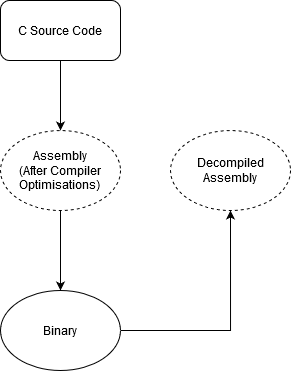
\includegraphics[width=\linewidth]{compilation.png}
    \caption{The static analysis options after compilation.}
    \label{fig:analysis}
\end{figure}

% TODO: Include figure of this problem

% TODO: Symbol table.

\subsection{Related Work}
In safety-critical real-time software such as flight control systems, it is required to analyse the \textit{Worst Case Execution Time} (WCET). This kind of analysis can be conducted using static analysis tools to estimate safe upper bounds. In the case of AbsInt's aiT tool this analysis is conducted alongside compiler annotations to assist where loop bounds cannot be computed statically. In these cases, the user can provide annotations to guide the analysis tools \cite{schommer2018embedded}. This tool builds on an existing annotation mechanism that exist in CompCert, a C compiler that has been formally verified for use in life-critical and mission-critical software \cite{compcert}\cite{leroy2016compcert}. CompCert annotations are not limited to WCET analysis. A general mechanism for attaching free-form annotations that propagate through to assembly files can be achieved with CompCert. This approach is able to reliably transmit compiler annotations through to binary through method calls which are carried through compilation and the linked executable without using external annotation files. CompCert prints annotation strings as a comment in the generated assembly code, and an additional tool is used to parse these comments and generate annotations. However, due to its treatment as an external function, annotations cannot be placed at the top level of a compilation unit, unlike a variable declaration. Compiler optimisations can additionally cause further issues when trying to preserve annotations through compilation. If dead code is eliminated, annotations associated with that code can be lost as well. Extra care needs to be taken to avoid these optimisations destroying links between properties and the code they refer to during such transformations.

\label{subsec:relatedWorkCompCert}
TODO: Include further documentation on how to use Compiler \& inline assembly
% https://compcert.org/man/manual006.html#sec112

A similar approach to CompCert is used by The ENTRA (Whole-Systems ENergy TRAnsparency). As part of providing a common assertion language, pragmas are used to propagate information through to comments in the assembler files. Information is retained in LLVM IR and ISA representations. However, these annotations are not stored in the final binary and thus comments must be extracted from assembler files \cite{eder2013common}.

Vu et al. \cite{vu2020secure} explore capturing and propagating properties from the source code level though though lowering passes and intermediate representations. Their goal was to maintain these properties to binary through aggressive compiler optimisations. As compilers only care about functional correctness, they have no notion of the link between properties and the code it refers to. Thus, there is no way to constrain transformations to preserve this link or to update these properties after the transformation. As such, they approached the problem to create a generic solution, modifying a LLVM compiler with virtually no optimisation changes. This was done by creating a library in LLVM. The properties were stored in strings, and these strings were parsed to build a list of observed variables and memory location. A LLVM pass was inserted to store all these properties in metadata. After each optimisation pass, a verification pass was inserted to check the presence of metadata representing the properties, variables amd memory locations. If an optimisation pass had cased the verification to fail the programmer would then be notified, to which they could annotate differently or disable the optimisation.


\clearpage
% !TeX root = ./report.tex
\chapter{Approach}
The approach was set out by first analysing existing methods of preserving annotations through intermediate representations. These include the:
\begin{itemize}
    \item the compCert Verified C Compiler, 
    \item GNU Extension for Extended Inline Assembly, and
    \item modifying the LLVM compiler to preserve annotations throughout intermediate representations.
\end{itemize}

Each of these approaches will be analysed individually for viability across each of the test cases outlined in section \ref{sec:testCases}. For approaches that pass all necessary test cases, a further analysis will be conducted into its suitability and development of any necessary tools to assist in the preservation technique, as outlined in sections \ref{sec:qualityAnalysis} and \ref{sec:toolDevelopment}. Finally, an analysis on the runtime efficiency of the program will be conducted to assess the success of the annotations with various levels of optimisation. The approach for this analysis is outlined in \ref{sec:runtimeEfficiencyOptimisation}.

\section{Test Cases}
\label{sec:testCases}
A suite of test C programs (See Appendix \ref{app:testPrograms}) were created to assist in guiding the process of evaluating each approach as a possible means of preserving annotations. Each program has inline comments documenting the annotation that should be preserved and its location within the program. Additionally, each program aims to test a separate element required to perform a static wpif analysis. Namely, these are to preserve the following through to the assembly output:

\begin{enumerate}
    \item comments,
    \item simple and complex variables (e.g. struct elements and volatile global variables),
    \item security policies,
    \item predicates on the initial state, and
    \item loop invariants.
\end{enumerate}

Each test was conducted to assess the viability of each approach of preserving annotations. If the approach cannot preserve all the required annotations described in the aforementioned list, then it is not viable for a wpif analysis and another technique must be explored.

The justification for each of the test files are as follows:

\miniheading{comment.c}
This test case is primarily a stepping stone to testing more complex scenarios. Here we have a generic comment "critical comment" and we are looking to preserve it through to the assembly. As well as preserving the comment itself, the location of the comment within the source code is to be preserved.

\miniheading{variable.c}
The test file \textit{variable.c} builds off \textit{comment.c}, however, we are additionally looking to preserve annotations about local variables within the program. Here multiple variable types are tested:

\begin{itemize}
    \item int,
    \item char,
    \item unsigned int,
    \item short,
    \item long,
    \item float, and
    \item double.
\end{itemize}

With each of these variables their type data is included as an annotation. This test is particularly interesting as with higher levels of optimisation we can observe how the annotations behave when a variable is optimised out.

\miniheading{volatile.c}
This test program looks at how the technique handles volatile variables. A variable declared as volatile tells the program its value could change unexpectedly. This is especially important when dealing with concurrent programs. If the technique cannot handle volatile variables it is unable to be used for a wpif analysis.

\miniheading{loop.c}
This test program tests how the annotator handles loops and loop invariants. It contains security policies, predicates on the initial state and loop invariants.

\miniheading{rooster.c}
The test program, \textit{rooster.c} delves into a more complex program, combining several features of the previous tests. It contains annotations within functions and global variables.

\miniheading{password.c}
This program tests how annotations are preserved within structs, a user-defined data type. Additionally, \textit{password.c} is a more complex program with multiple functions.

\miniheading{deadStoreElimination.c}
Testing dead store elimination is a bit more complex, as it requires comparing the compiled output before and after compiler optimisations are turned on. Here, the test program simulates the program described in section \ref{sec:compilersSecurity}.

\miniheading{pread.c}
The program \textit{pread.c} is a culmination of all the previous test cases, and is similar to \textit{loop.c}, however, the global variables within it are volatile. It requires all the necessary components for a wpif analysis.

\section{Quality Analysis}
\label{sec:qualityAnalysis}
Although a method of preserving c annotations may be able to successfully pass all the test cases, it is important to avoid modifying the assembly instructions. The reason for performing a static analysis on the compiled output is due to the optimisations performed by the compiler. As such, it is important to ensure that preserved annotations do not remove or undo any optimisations that may have been performed by the compiler. 

The methodology for testing quality in this manner is to compare the compiled assembly output for a program with annotations on to the compiled assembly output for the same program without annotations. If unnecessary assembly instructions have been added, it is indicative that the annotations has modified the program in unintended ways. 

\section{Efficiency and Optimisation}
\label{sec:runtimeEfficiencyOptimisation}
In the case that the annotations have introduced additional statements into the compiled assembly output, understanding the extent of these changes is important. Here, a efficiency analysis can be conducted on the assembly. Using big O notation, an upper bound can be placed on the program. Doing so allows for a comparison of the efficiency of the annotated and non-annotated assembly. 

Let \(A(n)\) be the function describing the annotated assembly, and \(B(n)\) be the function describing the non-annotated assembly. Then,

\[A(n) \in \Theta(g(n))\]
\[B(n) \in \Theta(h(n))\]

If the non-annotated assembly has a lower bound than the annotated assembly, such that

\[h(n) \in O(g(n)), and\]
\[g(n) \notin O(h(n))\]

then the annotations have modified the program in a way that reduces runtime efficiency. It is important to detect when this has happened, as it indicates the annotations have reversed the intended compiler optimisations.

In the case where the annotation process has resulted in additional assembly instructions inserted into the compiled output, however, they do not reduce runtime efficiency in terms of big O notation, a empirical analysis of the runtime duration of a program can be conducted to assess the disadvantage of the annotated program.

\section{Tool Development}
\label{sec:toolDevelopment}
In cases where it is appropriate, a tool may be developed to assist in the annotating process. This tool may either:
\begin{itemize}
    \item assist in the annotating process,
    \item verify the correctness of the annotations, or
    \item perform additional analysis on the compiled output.
\end{itemize}
If the approach of modifying the LLVM compiler is pursued, developing such a tool to assist the annotating process will be necessary.
% !TeX root = ./report.tex
\section{Execution}
Experimentation began with the CompCert compiler and the provided assembly annotation tools, outlined in section \ref{subsec:compCert}. It was found that the CompCert compiler could not handle all cases necessary for the wpif analysis, specifically volatile variables. As a result, the testing moved on to other techniques. Following this, the GNU C extension for inline assembly was explored as a possibility to preserve annotations in C in section \ref{subsec:inlineAssembly}. This technique prevailed and was found to be excellent in handling assembly annotations by injecting comments in to the compiled assembly output. This technique was enhanced by developing a python program to inject inline assembly into the source C files to allow for enhanced analysis and furthermore avoids restricting the program to GNU extension supporting compilers. As a result of the success, modifying the compiler was not explored due to success documented in other research such as the work conducted by Vu et al. \cite{vu2020secure}. This allowed for further development and improvement of the inline assembly method.

\subsection{CompCert AIS Annotations}
\label{subsec:compCert}
CompCert is unfortunately not a free tool, however, for research purposes it can be used freely. The specifications of the CompCert install can be seen in Table \ref{tab:compcertInstall}. 

\begin{table}
    \begin{center}
        \begin{tabularx}{\linewidth} { 
            | >{\hsize=.7\hsize\linewidth=\hsize}X 
            | >{\hsize=1.3\hsize\linewidth=\hsize}X  | }
            \hline
            OS Name & Ubuntu 20.04.2 LTS \\
            \hline
            OS Type & 64-bit \\
            \hline
            Processor & Intel® Core™ i7-6700K CPU @ 4.00GHz × 8 \\
            \hline
            Instruction Set & x86-64 \\
            \hline
            \raggedright
            CompCert Version & The CompCert C verified compiler, version 3.7 \\
            \hline
        \end{tabularx}
    \end{center}
    \caption{CompCert install specifications}
    \label{tab:compcertInstall}
\end{table}

Testing was initially conducted using the \textit{comment.c} test file. The goal is to propagate the comment down to assembly where it can be used and interpreted. To do so, the comment in the source code needs to be replaced with a call to generate an annotation in the compiled assembly. Fortunately, with the CompCert compiler, this functionality is builtin. This assembly annotation is created through the use of the \texttt{\_\_builtin\_annot} function described in \ref{subsec:relatedWorkCompCert}. The following builtin annotation was placed in line 2, within the main function in \textit{comment.c}.

\lstinputlisting[firstnumber=2, firstline=2, lastline=2, caption=comment.c]{source/compCert/comment.c}

Within this annotation, \code{\%here} is used to represent the location within the program. If the location is not important, \code{\%here} can be omitted. The comment, \code{"Critical Comment"}, has been included to represent some kind of critical comment that is required to conduct a static analysis on the output. To compile the source to assembler only the following command was used:

\begin{lstlisting}[numbers=none]
$ ccomp comment.c -O0 -S
\end{lstlisting}

Here -O0 is used to specify to perform no optimisations during compilation. The full compiled output can be seen in Appendix \ref{app:compCertOutput}. Below is a snippet of the compiled assembly.

\lstinputlisting[firstnumber=16, firstline=16, lastline=24, caption=comment-O0.s]{source/compCert/comment-O0.s}

The annotation is stored within assembler directives. Assembler directives are not a part of the processor instruction set, however, are a part of the assembler syntax. Assembler directives all start a period (.). On line 19 a new section has been created, named \texttt{"\_\_compcert\_ais\_annotations"}. Following the declaration of the section is an ascii string, locating the source of the annotation within the source program \textit{comment.c}. Line 23 provides the comment we aimed to preserve with our annotation. Thus, CompCert has shown an initial success in preserving annotations in the form of comments.

Additionally, one major benefit of compCert annotations is that they do not modify the source program, as they are inserted at the end of the program as an assembler directive metadata.

When experimenting with annotated variables, the first issues began to arise. The test file \textit{variable.c} contains several variables with their types to preserve to assembly. The annotations behaved as expected for the types:

\begin{itemize}
    \item int,
    \item char,
    \item short, 
    \item long, and
    \item any signed or unsigned variations of the above mentioned types.
\end{itemize}

However, the CompCert annotations does not support floating point types. Upon compiling \textit{variable.c} the following errors were generated.

\begin{lstlisting}[numbers=none]
variable.c:13: error: floating point types for parameter '%e1' are not supported in ais annotations
variable.c:15: error: floating point types for parameter '%e1' are not supported in ais annotations
2 errors detected.
\end{lstlisting}

This result shows that it is impossible to use the CompCert embedded program annotations for floating point types, vastly restricting its potential use as a technique for a wpif analysis.

It was discovered soon after that the CompCert annotations are unable to handle volatile variables, generating the follow error upon compiling \textit{volatile.c}.

\lstinputlisting[numbers=none]{source/compCert/volatile-O0.s}

Unfortunately, this result shows that the CompCert AIS annotations approach is not suitable for wpif analysis. The wpif analysis requires use of volatile variables. This is because the primary purpose of the wpif technique is to verify security policy across concurrent programs. Shared variables within concurrent programs can change at any time, and as such it is imperative that shared variables are marked as volatile. As the CompCert AIS annotations cannot handle volatile variables, annotations required for wpif analysis cannot be generated.

Aside from the aforementioned issues, the CompCert AIS annotations performed excellently in generating annotations. The location of global variables in memory are easily identified, as shown in \textit{rooster.c}. The CompCert AIS annotations must be placed within a method and called as if it was its own function. This creates some confusion when dealing with global variables. However, placing annotations on global variables at the start of main is a perfectly valid method of preserving these annotations. As the location of the annotation within the program is no longer important, the \code{\%here} format specifier can be omitted.

\lstinputlisting[firstline=84, firstnumber=84, caption=rooster-O0.s]{source/compCert/rooster-O0.s}

From \textit{rooster.c}, the comment "CRITICAL COMMENT" has been annotated from lines 88 to 91, and the comment "EXCEPTIONAL" has been annotated from lines 99 to 102. Most notably, the global variable \code{goose} has been annotated from lines 92 to 98. Reconstructed, the string \code{"L(mem(goose, 4)) = medium"} has been preserved. Thus, the CompCert annotations can successfully preserve annotations on global variables.


Another interesting problem faced when working with CompCert AIS annotations is found when working with structs. If the programmer wants to annotate a member of a struct for all structs of that type, each instance of that type of struct must be annotated when using CompCert AIS annotations. This is because CompCert treats \code{\_\_builtin\_ais\_annot()} as a call to an external function. As such, an annotation cannot be created from outside a method, similar to when dealing with global variables. An example of this process can be seen in \textit{password.c}. Within the program, each instantiation of the struct \code{user\_t} requires another annotation.

\lstinputlisting[firstline=17, firstnumber=17, lastline=33, caption=password.c, language=C]{source/compCert/password.c}



\subsubsection{Quality Analysis}
- TODO: How good is the compcert yo

\subsection{Inline Assembly}
\label{subsec:inlineAssembly}
TODO: Inline assembly techniques

\subsection{CompCert Builtin Annotations}

\subsection{LLVM Compiler Modification}
the final technique of modifying the LLVM compiler was not experimented on. This was primarily due to two reasons. To begin with, the primary objective of this thesis is to explore techniques that do not modify the compiler, and instead work alongside the functionality of the compiler to preserve annotations. It is well known and documented that modifying the compiler to preserve annotations is possible and successful, as in the case of Vu et al. \cite{vu2020secure} Additionally, earlier success through the technique of using inline assembly allowed for more time to be allocated to exploring and improving this technique, as seen in \ref{subsec:inlineAssembly}. Therefore, evaluating compiler modification for static analysis purposes was not performed in this research.

% TODO: 
% - Inline assembly
% - Source Code documentation
% - Speed Comparison Normal, CompCert, Inline Ass

% Recommendations
% - Improve tool -> Remove unnecessary move statements. More enhanced check of validity. Testing output with wpif techniques
% - Delve into modifying compiler techniques
% - 
\clearpage
\printbibliography
\clearpage

% !TeX root = ./report.tex

\onecolumn
\begin{appendices}
\addtocontents{toc}{\protect\setcounter{tocdepth}{0}}
\section{Test C Programs}
\label{app:testPrograms}

\subsection{comment.c}
\lstinputlisting[language=C]{source/comment.c}

\subsection{variable.c}
\lstinputlisting[language=C]{source/variable.c}

\subsection{volatile.c}
\lstinputlisting[language=C]{source/volatile.c}

\subsection{loop.c}
\lstinputlisting[language=C]{source/loop.c}

\subsection{rooster.c}
\lstinputlisting[language=C]{source/rooster.c}

\subsection{password.c}
\lstinputlisting[language=C]{source/password.c}

\subsection{deadStoreElimination.c}
\lstinputlisting[language=C]{source/deadStoreElimination.c}

\subsection{pread.c}
\lstinputlisting[language=C]{source/pread.c}

\section{CompCert Annotated C Programs}
\label{app:compCertC}
\subsection{comment.c}
\lstinputlisting[language=C]{source/compCert/comment.c}

\subsection{variable.c}
\lstinputlisting[language=C]{source/compCert/variable.c}

\subsection{volatile.c}
\lstinputlisting[language=C]{source/compCert/volatile.c}

\subsection{loop.c}
\lstinputlisting[language=C]{source/compCert/loop.c}

\subsection{rooster.c}
\lstinputlisting[language=C]{source/compCert/rooster.c}

\subsection{password.c}
\lstinputlisting[language=C]{source/compCert/password.c}

\subsection{deadStoreElimination.c}
\lstinputlisting[language=C]{source/compCert/deadStoreElimination.c}

\subsection{pread.c}
\lstinputlisting[language=C]{source/compCert/pread.c}

\section{CompCert Assembly Output}
\label{app:compCertAssembly}
\lstset{language=[x64]Assembler}
\subsection{comment-O0.s}
\lstinputlisting{source/compCert/out/comment-O0.s}
\subsection{comment-O3.s}
\lstinputlisting{source/compCert/out/comment-O3.s}

\subsection{variable-O0.s}
\lstinputlisting{source/compCert/out/variable-O0.s}
\subsection{variable-O3.s}
\lstinputlisting{source/compCert/out/variable-O3.s}

\subsection{volatile-O0.s}
\lstinputlisting{source/compCert/out/volatile-O0.s}
\subsection{volatile-O3.s}
\lstinputlisting{source/compCert/out/volatile-O3.s}

\subsection{loop-O0.s}
\lstinputlisting{source/compCert/out/loop-O0.s}
\subsection{loop-O3.s}
\lstinputlisting{source/compCert/out/loop-O3.s}

\subsection{rooster-O0.s}
\lstinputlisting{source/compCert/out/rooster-O0.s}
\subsection{rooster-O3.s}
\lstinputlisting{source/compCert/out/rooster-O3.s}

\subsection{password-O0.s}
\lstinputlisting{source/compCert/out/password-O0.s}
\subsection{password-O3.s}
\lstinputlisting{source/compCert/out/password-O3.s}

\subsection{deadStoreElimination-O0.s}
\lstinputlisting{source/compCert/out/deadStoreElimination-O0.s}
\subsection{deadStoreElimination-O3.s}
\lstinputlisting{source/compCert/out/deadStoreElimination-O3.s}

\subsection{pread-O0.s}
\lstinputlisting{source/compCert/out/pread-O0.s}
\subsection{pread-O3.s}
\lstinputlisting{source/compCert/out/pread-O3.s}

\section{CompCert Annotated Assembly Output}
\label{app:compCertAnnotatedAssembly}
\lstset{language=[x64]Assembler}
\subsection{comment-O0.s}
\lstinputlisting{source/compCert/annotated/comment-O0.s}
\subsection{comment-O3.s}
\lstinputlisting{source/compCert/annotated/comment-O3.s}

\subsection{variable-O0.s}
\lstinputlisting{source/compCert/annotated/variable-O0.s}
\subsection{variable-O3.s}
\lstinputlisting{source/compCert/annotated/variable-O3.s}

\subsection{volatile-O0.s}
\lstinputlisting{source/compCert/annotated/volatile-O0.s}
\subsection{volatile-O3.s}
\lstinputlisting{source/compCert/annotated/volatile-O3.s}

\subsection{loop-O0.s}
\lstinputlisting{source/compCert/annotated/loop-O0.s}
\subsection{loop-O3.s}
\lstinputlisting{source/compCert/annotated/loop-O3.s}

\subsection{rooster-O0.s}
\lstinputlisting{source/compCert/annotated/rooster-O0.s}
\subsection{rooster-O3.s}
\lstinputlisting{source/compCert/annotated/rooster-O3.s}

\subsection{password-O0.s}
\lstinputlisting{source/compCert/annotated/password-O0.s}
\subsection{password-O3.s}
\lstinputlisting{source/compCert/annotated/password-O3.s}

\subsection{deadStoreElimination-O0.s}
\lstinputlisting{source/compCert/annotated/deadStoreElimination-O0.s}
\subsection{deadStoreElimination-O3.s}
\lstinputlisting{source/compCert/annotated/deadStoreElimination-O3.s}

\subsection{pread-O0.s}
\lstinputlisting{source/compCert/annotated/pread-O0.s}
\subsection{pread-O3.s}
\lstinputlisting{source/compCert/annotated/pread-O3.s}

\section{Inline Assembly Annotated C Programs}
\label{app:InlineC}
\subsection{comment.c}
\lstinputlisting[language=C]{source/inline/comment.c}

\subsection{variable.c}
\lstinputlisting[language=C]{source/inline/variable.c}

\subsection{volatile.c}
\lstinputlisting[language=C]{source/inline/volatile.c}

\subsection{loop.c}
\lstinputlisting[language=C]{source/inline/loop.c}

\subsection{rooster.c}
\lstinputlisting[language=C]{source/inline/rooster.c}

\subsection{password.c}
\lstinputlisting[language=C]{source/inline/password.c}

\subsection{deadStoreElimination.c}
\lstinputlisting[language=C]{source/inline/deadStoreElimination.c}

\subsection{pread.c}
\lstinputlisting[language=C]{source/inline/pread.c}

\section{Inline Assembly Annotated Assembly Output}
\label{app:inlineAnnotatedAssembly}
\lstset{language=[x64]Assembler}
\subsection{comment-O0.s}
\lstinputlisting{source/inline/annotated/comment-O0.s}
\subsection{comment-O3.s}
\lstinputlisting{source/inline/annotated/comment-O3.s}

\subsection{variable-O0.s}
\lstinputlisting{source/inline/annotated/variable-O0.s}
\subsection{variable-O3.s}
\lstinputlisting{source/inline/annotated/variable-O3.s}

\subsection{volatile-O0.s}
\lstinputlisting{source/inline/annotated/volatile-O0.s}
\subsection{volatile-O3.s}
\lstinputlisting{source/inline/annotated/volatile-O3.s}

\subsection{loop-O0.s}
\lstinputlisting{source/inline/annotated/loop-O0.s}
\subsection{loop-O3.s}
\lstinputlisting{source/inline/annotated/loop-O3.s}

\subsection{rooster-O0.s}
\lstinputlisting{source/inline/annotated/rooster-O0.s}
\subsection{rooster-O3.s}
\lstinputlisting{source/inline/annotated/rooster-O3.s}

\subsection{password-O0.s}
\lstinputlisting{source/inline/annotated/password-O0.s}
\subsection{password-O3.s}
\lstinputlisting{source/inline/annotated/password-O3.s}

\subsection{deadStoreElimination-O0.s}
\lstinputlisting{source/inline/annotated/deadStoreElimination-O0.s}
\subsection{deadStoreElimination-O3.s}
\lstinputlisting{source/inline/annotated/deadStoreElimination-O3.s}

\subsection{pread-O0.s}
\lstinputlisting{source/inline/annotated/pread-O0.s}
\subsection{pread-O3.s}
\lstinputlisting{source/inline/annotated/pread-O3.s}

\end{appendices}
\end{document}
